\section{Develop the Application}
\label{create_flask_image_server}

In this section, we will develop a  small utility application based on the  Flask, \url{http://flask.pocoo.org/}, microframework that will allow us
to see on our computeer what the Raspberry Pi robot sees via the Pi camera.
Figure \ref{image_server_app}, shows a schematic of our application.

\begin{figure}[!htb]
\begin{center}
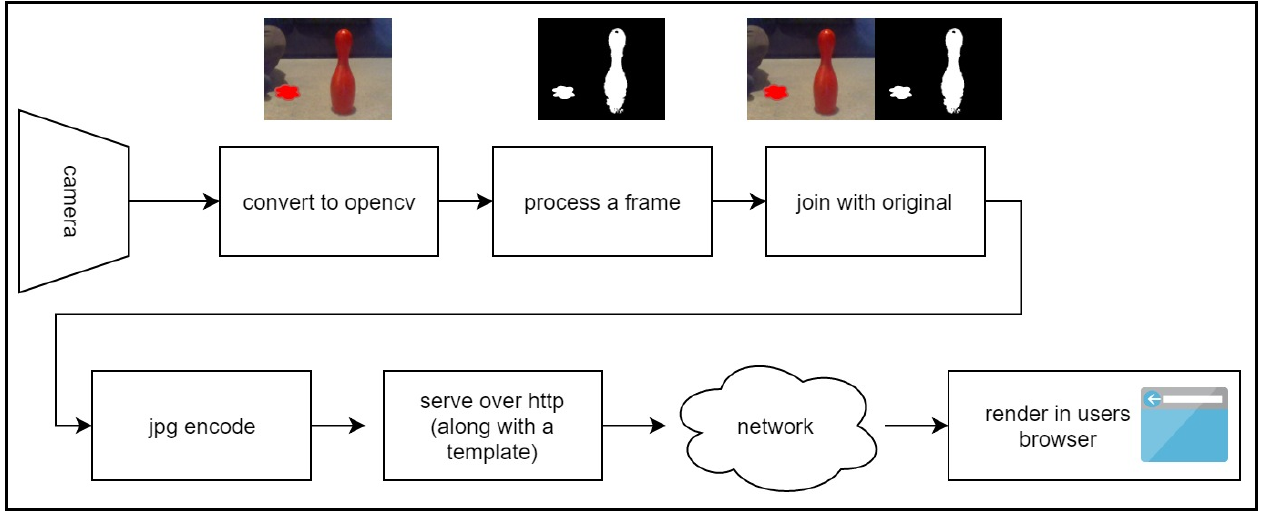
\includegraphics[scale=0.280]{img/raspberrypi/image_server_app.jpeg}
\end{center}
\caption{The image server app.}
\label{image_server_app}
\end{figure}


\begin{framed}
\begin{remark}

The Python code in this section is in  the \url{simulator/odisseus_v2/image_server} directory.
\end{remark}
\end{framed}

To begin with, login to Raspberry Pi board via Putty and install Flask by issuing

\begin{lstlisting}
pip3 install Flask
\end{lstlisting}

Then install the \lstinline{PiCamera} python framework \url{https://picamera.readthedocs.io/en/release-1.13/} 

\begin{lstlisting}
sudo pip3 install picamera[array] numpy
\end{lstlisting}

Once this is done make sure that the Pi camera is enabled and works properly. You can do so by getting a static image

\begin{lstlisting}
raspistill -o test.jpg
\end{lstlisting}

You can use FileZilla to easily transfer the image from Raspberry Pi to your PC.


Let us now develop the application. This utility application is organized around the following files

\begin{itemize}
\item \lstinline{pi_camera_stream.py}
\item \lstinline{image_server.py}
\item \lstinline{image_server.html}
\item \lstinline{conf.py}
\item \lstinline{picam_mock.py}
\end{itemize}

\lstinline{conf.py} simply introduces some configuration parameters

\begin{lstlisting}
"""
Configuration parameters for Odisseus V2
"""

import cv2

ON_RASP_PI:bool = False
SCREEN_SIZE:tuple = (320, 240)
ENCODE_PARAMS = [int(cv2.IMWRITE_JPEG_QUALITY), 90]
\end{lstlisting}

The \lstinline{pi_camera_stream.py} script provides the workhorse of our application

\begin{lstlisting}
from conf import ON_RASP_PI
from conf import SCREEN_SIZE
from conf import ENCODE_PARAMS

if ON_RASP_PI == True:
    from  picamera.array import PiRGBArray
    from  picamera import PiCamera
else:
    from picam_mock import  PiRGBArray
    from picam_mock import PiCamera
import cv2
import time

size = SCREEN_SIZE
encode_param = ENCODE_PARAMS

def setup_camera(rotation = 0.0)->PiCamera:
    """
    Set up the camera
    """

    camera = PiCamera()
    camera.resolution = size
    camera.rotation = rotation
    return camera


def start_stream(camera: PiCamera):

    image_storage = PiRGBArray(camera, size=size)

    # set up the stream of data. 'bgr' 
		# is the format OpenCV stores color data
    # use_video_port, which, when set to true, 
		# results in a reduction in
    # image quality in exchange for 
		# faster production of frames.

    cam_stream = camera.capture_continuous(image_storage=image_storage, 
format='bgr', use_video_port=True)

    for raw_frame in cam_stream:
        yield raw_frame.array

        # reset so that we can hold the next image
        image_storage.truncate(0)


def get_encoded_bytes_for_frame(frame)->str:
    """
    Encodes an image with OpenCV
    """

    result, encoded_img = cv2.imencode('.jpg', frame, encode_param)
    return encoded_img.tostring()

def frame_generator(rotation):
    """
    Main video feed
    """
    camera = setup_camera(rotation=rotation)

    # allow the camera to warm up
    time.sleep(0.1)

    for frame in start_stream(camera=camera):
        encode_bytes = get_encoded_bytes_for_frame(frame)
        yield (b'--frame\r\n'
               b'Content-Type: image/jpeg\r\n\r\n' + 
encode_bytes + b'\r\n')
\end{lstlisting}

\lstinline{image_server.py} allows us to launch the Flask application

\begin{lstlisting}
from flask import Flask
from flask import render_template
from flask import Response

from .pi_camera_stream import frame_generator


app = Flask(__name__)

@app.route('/')
def index():
    return render_template('image_server.html')


@app.route('/display')
def display():
    return  Response(frame_generator(rotation=0.0), 
mimetype='multipart/x-mixed-replace; boundary=frame')


app.run(host='0.0.0.0', debug=True, port=5001)
\end{lstlisting}

The application uses the \lstinline{templates/image_server.html} template

\begin{lstlisting}
<!DOCTYPE html>
<html lang="en">
<head>
    <meta charset="UTF-8">
    <title>Robot Image Server</title>
</head>
<body>
    <h1>Robot Image Server</h1>
    <img src="{{ url_for('display') }}">
</body>
</html>
\end{lstlisting}


\begin{framed}
\begin{remark}

Note that the \lstinline{image_server.html} should be in the \lstinline{templates/} directory.
\end{remark}
\end{framed}

Finally, the \lstinline{picam_mock.py} is used for testing purposes and not currently needed.

Transfer the files on Raspberry Pi and  run the Flask application

\begin{lstlisting}
export FLASK_APP=image_server.py
flask run
\end{lstlisting}

Then navigate to the following url on your PC; \url{raspberrypi.local:5001} and view the image that 
is captured by the Pi camera and sent over the internet by our small utility application.
 





